% Energy Bench: methodology preprint.
% Build: latexmk -pdf energybench_methodology.tex. Table rows and elo_live.dat are generated from the scores by
% scripts/research/preprint_results.py (numbers as of 15 Oct 2026).
\documentclass[11pt,a4paper]{article}
\usepackage[T1]{fontenc}
\usepackage[utf8]{inputenc}
\usepackage{libertinus}
\usepackage[scaled=0.86]{beramono}
\usepackage[margin=2.5cm]{geometry}
\usepackage{microtype}
\usepackage{amsmath,amssymb}
\usepackage{booktabs}
\usepackage{threeparttable}
\usepackage{tabularx}
\newcolumntype{Y}{>{\raggedright\arraybackslash}X}
\usepackage{xcolor}
\usepackage{tikz}
\usetikzlibrary{arrows.meta,positioning,decorations.pathreplacing}
\usepackage{pgfplots}
\pgfplotsset{compat=1.18}
\usepackage[numbers,sort&compress]{natbib}
\usepackage[hidelinks]{hyperref}
\usepackage{enumitem}
\setlist{itemsep=2pt,topsep=4pt}

\definecolor{navy}{HTML}{0B1F3A}
\definecolor{accent}{HTML}{C8102E}
\definecolor{covc}{HTML}{2E6DB4}
\definecolor{histc}{HTML}{8A8F98}
\newcommand{\m}[1]{\texttt{#1}}

\title{\textbf{Energy Bench: a live, gate-aligned benchmark\\of day-ahead forecasts for European power markets}}
\author{Evgenii Genov\\[2pt]
\small Vrije Universiteit Brussel\\
\small\href{mailto:evgeny@foretec.be}{evgeny@foretec.be}}
\date{\small Methodology preprint, 21 October 2026\\
\href{https://energybench.foretec.co}{energybench.foretec.co} \quad\textperiodcentered\quad
\href{https://github.com/ujohn33/foretec-energy-bench}{github.com/ujohn33/foretec-energy-bench}}

\begin{document}
\maketitle

\begin{abstract}
\noindent
Comparisons of energy forecasting models usually rest on backtests, and backtests are easy to get subtly wrong: the
information that was available when a forecast would have been sold is replaced by whatever is convenient to download
later. Energy Bench removes the question by running every entry live. Each day at 11:30 CET/CEST, thirty
minutes before the single day-ahead coupling (SDAC) gate closes, every model forecasts the next delivery day's
day-ahead price, wind generation, solar generation and total load on the 15-minute market grid for six bidding zones
(BE, NL, FR, DE-LU, DK1, DK2), from data that was public at that moment, including frozen numerical weather prediction
(NWP) runs. Unlike existing live benchmarks, it runs every model itself on that one frozen, published information
set, so foundation models are compared with and without the same weather covariates under a real market deadline. A
forecast that is not locked before the gate is never scored. Actuals come from the transmission system
operators' (TSOs') publications with recorded provenance, explicit completeness rules and a revision check. Models
are compared on errors pooled per series relative to a same-quarter-hour-last-week baseline, and ranked by a
Bradley--Terry rating of all pairwise comparisons on the Elo scale, with a confidence interval from resampling issue
days. A separate view values each wind and solar forecast as the day-ahead revenue of a 100\,MW asset settled at
published imbalance prices. The field, 40 active entries, spans naive and climatological baselines, linear and
gradient-boosted models on the frozen weather ensemble, tabular neural networks, ten families of pretrained
time-series foundation models with and without covariates, ensembles of them, and the TSOs' own forecasts as
references. This paper
describes the protocol, data, scoring and ranking, and reports the first eighteen live days. Covariates roughly
halve the error of foundation models: on matched races, giving the same model the frozen weather table cuts its error
relative to the seasonal-naive baseline by 42--49\% for five of six model families (by 66--74\% on wind and 52--62\% on
solar), and a covariate-aware foundation model leads the standings. Used zero-shot, five of the six beat a LightGBM
model trained on the same inputs. The grid operators' own forecasts remain the bar: on the series they cover, the best
entries are level with the forecasts published before the gate on wind but behind on solar and load, and behind the
final forecasts published after it. A model enters the benchmark by pull request.
\end{abstract}

\section{Introduction}

Day-ahead forecasts of price, renewable generation and load are the inputs of every bidding decision on European
power markets, and claims about how well a given model makes them are rarely comparable. Three things go wrong in the
usual backtest. First, the information set drifts: a forecast nominally made at 11:30 is built from weather runs that
were published hours later, from actuals that were still provisional, or from a TSO forecast that only appears after
the gate. Second, the target drifts away from the market's: hourly values where the market now trades quarter-hours,
generation definitions that differ between data providers, actuals that were later revised. Third, nothing stops an
author from choosing the window, the baseline or the metric after seeing the results.

A fourth gap has opened with time-series foundation models. In operational energy forecasting, exogenous inputs are
the standard, not an option: wind and solar forecasts are built on numerical weather predictions, load forecasts on
temperature and calendar effects, and day-ahead price forecasts on forecasts of load, renewable infeed and fuel
cost~\cite{hongreview,weron,lago}. The grid operators' own forecasts, the industry reference, are NWP-driven, and the
energy forecasting competitions supplied weather forecasts as a matter of course~\cite{gefcom}. The benchmarks on which
foundation models are compared are, by contrast, mostly univariate. A model that forecasts tomorrow's solar output from
the last four weeks of solar output alone is being tested on a task no practitioner would set it, and a ranking built
that way says little about which model to deploy.

A live benchmark that hands every entry the same inputs closes these holes by construction. If the model runs at the
real cut-off, on the data really available, weather forecasts included, and its forecast is locked before the real gate, there is no look-ahead to argue about, and the record
accumulates one day at a time in public. The price is patience: a live record is short and its standings are noisy
on any given day. The design below takes that noise seriously rather than hiding it: errors are pooled before they
are normalised, ranks come with intervals, and only live forecasts are reported.

Energy Bench went live on 2~October 2026 with three zones (BE, NL, FR) and three targets; total load was added on
6~October and three zones (DE-LU, DK1, DK2) on 15~October.
The code and the configuration file that define the benchmark are versioned in a public repository. This paper
describes that configuration as of 21~October 2026 and the results to date.

\section{Related work}

\paragraph{Static benchmarks.} Forecasting competitions have shaped the field since the M-competitions~\cite{m4}; the
Monash archive~\cite{monash}, GIFT-Eval~\cite{gifteval} and fev-bench~\cite{fevbench} standardise the evaluation of
general-purpose and foundation time-series models on fixed datasets. In energy, the Global Energy Forecasting
Competitions~\cite{gefcom} posed realistic tasks as one-off events, and Lago et al.~\cite{lago} published an open
benchmark for day-ahead price forecasting with fixed splits and day-ahead exogenous forecasts for five markets. Fixed
datasets have two weaknesses for the present purpose. They describe a past regime, and energy systems change quickly;
and their test periods may have been seen, directly or through pretraining corpora, by the models they evaluate.
Retrospective energy studies also often leave the information set implicit: several price-forecasting studies use
ENTSO-E's day-ahead wind and solar forecasts as inputs although those are published only after 18:00 on $D-1$, six
hours after the auction closes~\cite{energyarena}.

\paragraph{Covariates.} The value of weather inputs in energy forecasting is long established. Wind and solar power
forecasting has been NWP-based since its beginnings, and the wind and solar tracks of GEFCom2014 gave every team ECMWF
forecasts~\cite{gefcom}; load forecasting rests on temperature, and the reviews of price forecasting single out
forecasts of load and renewable generation as the most informative exogenous drivers~\cite{weron,lago,hongreview}.
Foundation models have only recently gained the means to use such inputs: Chronos-2, TimesFM, TiRex-2 and the t0
models accept known-future covariates, by different mechanisms and with different success. Whether and how much they
benefit is an empirical question that a univariate benchmark cannot answer, and it is the question an operational
user needs answered first.

\paragraph{Live benchmarks.} Two recent platforms evaluate forecasts made before the outcome exists, and each
leaves open a question that Energy Bench is built to answer.

TS-Arena~\cite{tsarena} implements a forecast pre-registration protocol for time-series foundation models: a round
hands out each series' history up to its last published value and closes registration before the next value is
recorded. Its 14 challenges draw on SMARD (German day-ahead price, load and generation), Gridstatus (US ISO hub
prices, load and generation) and Fingrid (Finland), at 15-minute resolution with a one-day horizon and hourly with a
three-day horizon, from a 1{,}000-step context. Models are scored by MASE and ranked by an online Elo rating whose
interval comes from replaying the rounds in random order. Two features limit what its rankings say about energy
forecasting. \emph{First, there are no covariates}: the foundation models forecast wind, solar and load from the
series' own history, without the weather forecast that any operational forecaster of those quantities would use, so
the benchmark measures a task no market participant faces, and a model's ability to exploit covariates, which in our
results halves the error of the same models (Section~\ref{sec:results}), is not measured at all. \emph{Second, the
information set is not tied to a market gate}: each round starts at the last published value, so the window follows
each source's publication delay rather than the market. A German price forecast registered on day $X$ starts after the
delivery day that cleared on $X$ and covers a later day than the next auction needs, and the generation and load
windows do not align with a delivery day at all. What a forecaster could have known at a decision time is therefore
not defined, and no forecast corresponds to a bid that could have been placed.

Energy-Arena~\cite{energyarena} is an open, API-based platform whose challenges are defined by their market deadline:
forecasts are submitted before 12:00 CET on $D-1$ for the whole next day, as point (RMSE), quantile (weighted interval
score) or ensemble (CRPS) forecasts, with leaderboards over rolling windows. It is gate-aligned, but it compares
\emph{submissions}, not models under common conditions. Participants run their own models on any inputs they have,
including proprietary weather, and describe them only if they choose to; they may also keep their forecasts hidden.
Since the information set cannot be verified, a difference on the leaderboard may reflect better data rather than a
better method, and entries cannot be reproduced. The platform names no reference models, so whether foundation models
are represented at all depends on who submits; and its wind, solar and load challenges cover only Austria and
Germany-Luxembourg (day-ahead prices extend to thirteen further zones). In industry, the Predico
platform~\cite{predico} scores live renewable forecasts submitted to Elia and 50Hertz against a real gate, for
enrolled forecasters and without publishing their inputs.

\paragraph{Positioning.} Energy Bench takes Energy-Arena's operational framing (the day-ahead gate defines the task)
and TS-Arena's pre-registration logic (only a forecast made before the outcome exists is free of leakage), and closes
the gaps between them by running every model itself. Each day it fetches one information set at the gate-aligned
cut-off, freezes and publishes it, and gives it to every entry: the information set is enforced rather than declared,
and any forecast can be reproduced from its archived inputs. Foundation models enter both without and with the same
frozen covariates, so the value of the weather is measured model by model rather than assumed away; all four targets
are forecast in six zones; and the grid operators' own forecasts, before and after the gate, serve as references. The
price is that entries are submitted as code rather than as forecasts, and proprietary data cannot be used.
Table~\ref{tab:compare} summarises the differences.

\begin{table}[t]
\centering\small
\caption{Live energy forecasting benchmarks compared, as described in their papers and on their websites (October 2026).}
\label{tab:compare}
\begin{tabularx}{\linewidth}{@{}>{\raggedright\arraybackslash}p{2.7cm}YYY@{}}
\toprule
& TS-Arena~\cite{tsarena} & Energy-Arena~\cite{energyarena} & Energy Bench (this paper) \\
\midrule
Task timing & from each series' last published value; no market gate & submission before the 12:00 day-ahead gate, whole next day & 11:30 cut-off, locked before the 12:00 gate, whole next day \\
Zones and targets & 14 challenges (SMARD, Gridstatus, Fingrid) & wind, solar, load: AT, DE-LU; price: 15 zones & price, wind, solar, load in each of BE, NL, FR, DE-LU, DK1, DK2 \\
Who runs models & participants (containers) & participants (API submissions) & the benchmark, from submitted code \\
Information set & series history only & anything before the gate; self-declared, unverified & frozen and published: history, three NWP models, load forecast, fuel \\
Covariates for foundation models & none & if a participant adds them & every foundation model with and without the same covariates \\
Foundation models & the focus of the field & none named; depends on submissions & ten families, and ensembles \\
Transparency & platform code public & method description and forecasts optional & code, inputs and forecasts public \\
Scores & MASE & RMSE, WIS, CRPS & MAE, RMSE, bias, pinball; relative to seasonal naive, pooled per series \\
Ranking & online Elo, replay bootstrap & per metric over rolling windows & Bradley--Terry Elo, day bootstrap \\
References & statistical baselines & optional benchmark models & baselines; the TSOs' forecasts before and after the gate \\
\bottomrule
\end{tabularx}
\end{table}

\section{The benchmark}

\subsection{Task}

For each zone $z \in \{\text{BE}, \text{NL}, \text{FR}, \text{DE-LU}, \text{DK1}, \text{DK2}\}$ and target $y \in
\{\text{price}, \text{wind}, \text{solar}, \text{load}\}$ (24 series), a forecast made on issue day $D-1$ covers
every quarter-hour of delivery day $D$ in local time: 96 values, or 92 and 100 on clock-change days. Price is the SDAC
day-ahead price (EUR/MWh); wind is onshore plus offshore generation, solar is solar generation and load is total load
(MW). Models return a point forecast and optionally the nine deciles $q_{0.1},\dots,q_{0.9}$. Danish load is published
only hourly, so DK load forecasts are scored on hourly averages of forecast and actual: detail that the actual cannot
resolve is neither rewarded nor penalised.

\subsection{Timeline and information set}

The benchmark day is defined by three clock times in CET/CEST (Figure~\ref{fig:timeline}). At the \emph{cut-off},
11:30 on $D-1$, a snapshot of everything public is taken and every model runs on it. The \emph{gate} is 12:00, the
SDAC gate closure: a live run that finishes after it is marked late and never scored, and a day's forecasts are
locked once written. Prices are scored on $D-1$ once the auction for $D$ has cleared (14:45 and 20:45 runs). Wind,
solar and load are scored at 07:00 on $D+1$ if every quarter-hour of $D$ has been published, otherwise at the next
scoring run once 95\% has.

\begin{figure}[t]
\centering
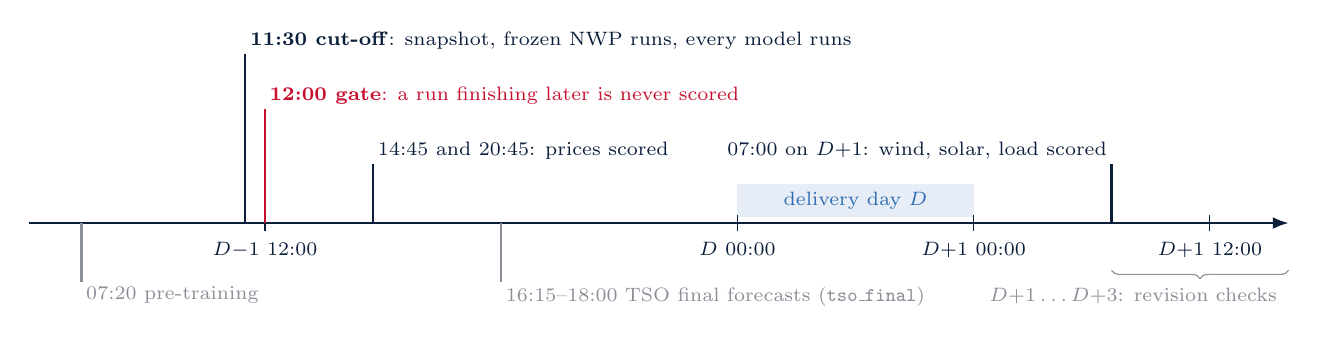
\begin{tikzpicture}[x=1cm,y=1cm,font=\scriptsize]
  % piecewise time axis: D-1 06:00..24:00 at 0.5 cm/h, day D at 0.125 cm/h, D+1 00:00..16:00 at 0.25 cm/h
  \fill[covc!12] (9,0.08) rectangle (12,0.5); \node[covc] at (10.5,0.29) {delivery day $D$};
  \draw[-{Latex[length=2mm]},thick,navy] (0,0) -- (16,0);
  \foreach \x/\l in {3/{$D{-}1$ 12:00},9/{$D$ 00:00},12/{$D{+}1$ 00:00},15/{$D{+}1$ 12:00}}
    {\draw[navy] (\x,-0.1) -- (\x,0.1); \node[below=2pt,navy] at (\x,-0.05) {\l};}
  \newcommand{\ev}[5]{\draw[#3,thick] (#1,0) -- (#1,#2); \node[anchor=#4,#3,inner sep=1.5pt] at (#1,#2) {#5};}
  \ev{2.75}{2.15}{navy}{south west}{\textbf{11:30 cut-off}: snapshot, frozen NWP runs, every model runs}
  \ev{3.0}{1.45}{accent}{south west}{\textbf{12:00 gate}: a run finishing later is never scored}
  \ev{4.375}{0.75}{navy}{south west}{14:45 and 20:45: prices scored}
  \ev{0.67}{-0.75}{histc}{north west}{07:20 pre-training}
  \ev{6.0}{-0.75}{histc}{north west}{16:15--18:00 TSO final forecasts (\m{tso\_final})}
  \ev{13.75}{0.75}{navy}{south east}{07:00 on $D{+}1$: wind, solar, load scored}
  \draw[decorate,decoration={brace,mirror,amplitude=3pt},histc] (13.75,-0.6) -- (16,-0.6)
    node[midway,below=3pt,anchor=north east,xshift=1.1cm,histc] {$D{+}1\dots D{+}3$: revision checks};
\end{tikzpicture}
\caption{One benchmark day (not to scale). Everything a model sees is fixed at the 11:30 cut-off; the forecast must
be locked before the 12:00 gate. The TSOs' final day-ahead wind and solar forecasts appear only after the gate and
enter as references.}
\label{fig:timeline}
\end{figure}

What a model may know at the cut-off is set per target. Prices: everything up to the end of $D-1$, which the auction
on $D-2$ published. Wind, solar and load: actuals up to the cut-off minus one hour of publication lag. Every model
receives the last 28 days of 15-minute history (the context). A model may train on longer history provided each
training row is built with exactly the history that was public at that row's own cut-off, and training never happens
inside the live window: models that retrain do so in a nightly catch-up or at 07:20, and a live run that finds no
trained model falls back to the latest earlier one rather than train. The TSOs' day-ahead renewable forecasts are not
an input: Regulation (EU) 543/2013~\cite{reg543} has them published by 18:00 on $D-1$, after the gate.

\subsection{Actuals and provenance}

The primary source is the ENTSO-E Transparency Platform~\cite{entsoe}, parsed from its XML: day-ahead prices (document
A44, the 15-minute SDAC prices), actual generation per production type (A75; wind as onshore B19 plus offshore B18,
solar B16) and actual total load (A65). ENTSO-E does not deliver every quarter-hour: alone it lacked 12\% of Belgian
and 2.6\% of French wind quarter-hours in September 2026. Gaps are filled from the TSOs' own open data (Elia for
Belgium, RTE éCO2mix for France), then from Energy-Charts as a last resort; where a TSO publishes finer data than it
sends ENTSO-E, the TSO comes first (Elia sends hourly wind and solar to ENTSO-E but publishes quarter-hours). Every
snapshot and every set of actuals records how many points came from each source, and the site shows it. Electricity
Maps' choice of sources served as the reference for the new zones, with one exception found in operation: ENTSO-E's
DK1 offshore wind covers only the parks registered there and has missed 0.3--0.5\,GW of new offshore capacity since
July 2026, so Danish wind has come from Energinet's real-time production data since delivery day 18 October (Danish
solar and load stay on ENTSO-E).

The Netherlands shows why provenance matters. ENTSO-E's Dutch series cover only what TenneT meters itself: solar at
about 1\% of the fleet (a capacity factor of 0.1\% over 20 September--7 October 2026, against 10.7\% in the national
estimate, 12.7\% in Belgium and 13.6\% in France), wind mostly offshore, and load net of embedded solar (about 6\,GW
against 17\,GW gross at a sunny midday). The Dutch wind, solar and load targets therefore come exclusively from NED,
the Nationaal Energie Dashboard backed by TenneT and the distribution operators, which publishes national estimates:
wind as onshore plus metered offshore, load as gross consumption as Elia and RTE report it. These series take no
fallback, since a gap is better than a mixture of definitions. Live forecasts made from the earlier ENTSO-E definition
(issue days up to 10 October for wind and solar, 11 October for load) are kept and shown but never scored. When a
series' definition changes but its earlier scores remain valid, the earlier actuals are locked: NED's offshore wind was
a park-by-park model through delivery day 12 October, 7--27\% above the metered output used since, and those days keep
their scores.

Actuals are \emph{frozen} the first time they are complete and scored from the frozen copy. For three days afterwards,
wind, solar and load are re-fetched at every scoring run; a change above 0.5\% of the day's energy re-freezes the
actuals and re-scores the day, and every check is logged. Prices are final at the auction. Between the gate and
scoring, the site shows the quarter-hours metered so far as provisional actuals, which are never scored.

\subsection{Covariates frozen at the cut-off}
\label{sec:cov}

Models that declare covariate inputs receive, per issue day, a table frozen at the cut-off and a log of what went
into it.

\paragraph{Weather.} Three independent global and regional NWP models, ICON-EU (DWD), GFS (NOAA) and IFS HRES (ECMWF),
are fetched run by run from the Open-Meteo single-runs archive~\cite{openmeteo}. A run is admitted only if its
initialisation is at most the cut-off minus a lag, the provider's measured publication delay plus a margin (3.5\,h for
ICON-EU, 7\,h for GFS and IFS); at 11:30 this admits the 06 UTC ICON-EU run and the 00 UTC GFS and IFS runs. Since 19 October a run must also be
complete: if any variable is less than 99\% filled over the delivery day, the fetch is retried and then falls back to
the previous cycle (Section~\ref{sec:limits}). Weather
is sampled at 153 capacity-weighted $k$-means centroids per zone and bucket (onshore wind, offshore wind, solar, and
population as the load proxy), built from public registers: Elia and the Belgian regions for BE, CBS for NL, ODRÉ's national register of
installations for FR, the Marktstammdatenregister for DE-LU and Energinet's capacity per municipality for DK1 and DK2. The table carries, per variable and bucket, each NWP model's capacity-weighted zone mean, and across the
three models the ensemble mean, spread and pairwise differences, so that disagreement can serve as a feature. Training
rows use the same rule day by day: the weather for a past delivery day comes from the runs that were available at that
day's own cut-off (the archive's previous-runs product is matched to the live lead time), so models train on forecasts
with the lead time they forecast with.

\paragraph{Load forecast.} ENTSO-E's day-ahead total load forecast (A65), which TSOs must publish two hours before the
gate.

\paragraph{Fuel cost.} TTF gas (ICE Dutch front month) and EU carbon allowance daily closes, a close counting only from
the end of its date, and the derived short-run marginal cost of a gas plant, $\text{TTF}/0.52 + 0.37\,\text{EUA}$
(EUR/MWh).

\subsection{Entries}

A model is a folder with a declarative \m{model.yaml}: a named sktime~\cite{sktime} estimator, a Python module, or a
subprocess script with its own environment, the route all foundation models take (each family loads its weights once
per day for all series). A model whose environment is missing is skipped and logged, not failed. The live run takes
10--20 minutes for the field on a four-core, 8\,GB server (17 minutes for 24 series on 15 October), against a
30-minute window; from 16 October two models run concurrently, each with half the CPU threads. Dropping a folder into
\m{models/} is the whole act of deployment: a nightly catch-up runs any new model over a fixed backtest window
(14 September -- 1 October 2026, shown on the site as a separate record and not used in this paper) and adds it to
the live run. The field on 21 October (Table~\ref{tab:field}) has 40 active entries.

\begin{table}[t]
\centering\small
\caption{The field, 21 October 2026. Covariate inputs are the frozen table of Section~\ref{sec:cov}.}
\label{tab:field}
\begin{tabularx}{\linewidth}{@{}p{3.1cm}X@{}}
\toprule
Group & Entries \\
\midrule
Baselines & \m{naive\_weekly} (same quarter-hour one week earlier; the reference of all relative errors),
\m{naive\_daily} (one day earlier), \m{climatology} (same local time of day within $\pm14$ calendar days, 2023 to
August 2026), \m{lin\_lags} and \m{lgbm\_lags} (ridge and LightGBM on lagged values of the series itself, two years of
training up to the end of the previous month, retrained monthly). \\
Covariate models & Ridge and LightGBM on the covariates and calendar, trained on the 28-day context
(\m{lin\_cov}, \m{lgbm\_cov}) or on two years (\m{lin\_cov\_2y}; \m{lgbm\_prod}, recency-weighted with a 120-day
half-life, retrained daily for price and load and monthly for wind and solar, solar trained on its capacity factor);
tabular neural networks on the \m{lgbm\_cov} inputs (\m{realmlp\_cov}~\cite{realmlp}, \m{tabm\_cov}~\cite{tabm};
backtest only so far). \\
Foundation models, history only & Chronos-2 and Chronos-Bolt~\cite{chronos}, TimesFM 2.5 and 3.0~\cite{timesfm},
Moirai~2~\cite{moirai}, TiRex and TiRex-2~\cite{tirex}, Toto, Sundial, TTM r2, Tabby and Tabby-Pretrain, Timestral
(Mistral AI), and the t0 alpha, beta and gamma releases of The Forecasting Company; all zero-shot. \\
Foundation models with covariates & \m{chronos2\_cov}, \m{timesfm3\_cov}, \m{t0\_alpha/beta/gamma\_cov} and
\m{tirex2\_cov} and \m{timestral\_cov} through their native known-future covariates; \m{timesfm25\_cov},
\m{tabby\_cov} and \m{tabby\_pretrain\_cov} through an in-context ridge regression (the foundation model forecasts
what the covariates do not explain). Moirai~2 and Toto with covariates were retired after the
trial runs: covariates made Moirai~2 worse, and Toto gained too little for its run time and memory. \\
Ensembles & Quarter-hourly medians of fixed members, point and each quantile separately: \m{ens\_fm}, the newest
history-only model of the five families that also have a native-covariate variant; \m{ens\_fm\_cov}, their five
covariate variants; \m{ens\_hybrid}, those five plus \m{lgbm\_prod}. Members are fixed by rule, not by score. \\
References & \m{tso\_cutoff}: the TSOs' forecasts as published before the gate (Elia's 11:00 day-ahead wind and solar
forecast for BE, NED's national forecast for NL fetched at the cut-off, and the ENTSO-E day-ahead load forecast);
live only, since a pre-gate vintage cannot be verified after the fact; ranked like any entry. \m{tso\_final}: the
final day-ahead wind and solar forecasts, published after the gate (Elia 18:00, RTE 16:15, ENTSO-E for DE-LU and DK,
NED in the evening for NL); shown, never ranked. \\
\bottomrule
\end{tabularx}
\end{table}

No TSO in France, Germany or Denmark publishes a day-ahead wind or solar forecast before the gate (RTE at 16:15, the
German TSOs and Energinet at 18:00 on $D-1$), so \m{tso\_cutoff} has wind and solar only for BE and NL. Classical
univariate models (ARIMA, ETS, Theta, CES, TBATS) were in the field in its first two weeks and were retired: on
15-minute data with a 96-step daily cycle and a 28-day context they were not competitive. Their records are kept but
no longer shown.

\subsection{Scoring}

For every forecast, issue day $d$ and series $s$ the benchmark records MAE, RMSE, bias and, for models with deciles,
the pinball loss averaged over the nine deciles,
\begin{equation}
\mathrm{PL} = \frac{1}{9\,T}\sum_{t=1}^{T}\sum_{\tau\in\{0.1,\dots,0.9\}} \max\!\big(\tau\,(y_t - q_{\tau,t}),\,(\tau-1)(y_t - q_{\tau,t})\big),
\end{equation}
with $T$ the scored quarter-hours of the day. Errors are compared across series of different scale by relating them
to the baseline \m{naive\_weekly}, and they are aggregated \emph{before} they are normalised: for model $m$, series
$s$ and the set $\mathcal{D}_{m,s}$ of issue days on which both $m$ and the baseline were scored,
\begin{equation}
\mathrm{RelMAE}_{m,s} = \frac{\sum_{d\in\mathcal{D}_{m,s}} \sum_t |e^{m}_{d,t}|}{\sum_{d\in\mathcal{D}_{m,s}} \sum_t |e^{\text{base}}_{d,t}|},
\qquad
\mathrm{RelRMSE}_{m,s} = \Big(\frac{\sum_{d,t} (e^{m}_{d,t})^2}{\sum_{d,t} (e^{\text{base}}_{d,t})^2}\Big)^{1/2}.
\end{equation}
A ratio of means rather than a mean of daily ratios keeps one calm day, on which the baseline happened to be nearly
right, from dominating the average. Over several series the per-series values are combined by the mean, the median or
the geometric mean; the site lets the reader switch. The geometric mean, used in the tables below, treats halving and
doubling the error symmetrically and penalises a model that fails on one series.

Three choices in these definitions deserve to be explicit, because each changes what ``best'' means.
\emph{Which summary of the predictive distribution is rewarded.} Absolute error is minimised by the median of the
predictive distribution and squared error by its mean~\cite{gneiting2011}; for skewed targets such as solar power or
spiking prices the two differ, and a model trained on quantile loss is not wrong to forecast the median. The field mixes
both: most foundation models report the median of their predictive quantiles (Chronos, TiRex, Moirai, Sundial, Toto),
while TimesFM and the LightGBM and ridge entries, fitted on squared error, report a conditional mean. The standings are
built on MAE and so reward the median; Rel.\ RMSE is shown next to it so that mean-oriented entries are not judged on
the other functional only, and bias is reported separately because neither accuracy measure distinguishes a systematic offset
from noise. \emph{Which benchmark is in the denominator.} Every scale-free error embeds a benchmark~\cite{hyndmankoehler}.
Energy Bench names it: the same quarter-hour one week earlier, a seasonal naive forecast that respects the daily and
weekly cycles of price and load and needs no fitting, evaluated on the same test days as the model rather than
in-sample, which is possible because every series has 96 scored values per day~\cite{davydenko}. For wind and solar it
is a weak benchmark, and relative errors well below one are expected there; the benchmark is a common unit, not a
claim about what is hard. \emph{How the dimensions are aggregated.} Errors are averaged over the 96 quarter-hours of
the delivery day and over issue days within a series, then across series with equal weight per series. Equal weight
is a choice: it asks which model forecasts best across forecasting problems, not where the most megawatts or euros
are; the forecast-value view (Section~\ref{sec:value}) gives the latter answer for wind and solar.

\subsection{Ranking}

A \emph{race} is one issue day and one series; its field is every model with a scored forecast in it. A model whose
run failed is left out of that race rather than ranked last (the run tracker on the site shows every failure), and a
model joins the races of the series it declares from the day it is added. Within a race every pair of models plays
one game, won by the lower relative error of the day (equal errors split the game). All games of the selected period
are fitted at once with a Bradley--Terry model~\cite{bradleyterry}, $P(i \text{ beats } j) = p_i/(p_i+p_j)$, by the
minorisation--maximisation algorithm of Hunter~\cite{hunter}, and reported on the Elo scale,
$\mathrm{Elo}_i = 1000 + 400\log_{10} p_i$, with the geometric mean of the strengths fixed at 1 so that 1000 is the
field's average. One virtual drawn game against an average opponent keeps the rating finite for a model that wins or
loses every game. Unlike a running Elo, the rating does not depend on the order of the races, and a win over a strong
model counts more than a win over a weak one; the same construction underlies the Chatbot Arena
leaderboard~\cite{chatbotarena}.

The 95\% interval is the 2.5th--97.5th percentile of 200 refits on issue days drawn with replacement. Days rather than
races are resampled because all races of a day share the same weather and tend to be won and lost together.
Overlapping intervals mean the order of two models is not settled. Any pairwise rating is relative to the field: a model's score depends on whom it
played, and several near-identical entries (three releases of one model family, say) take wins from each other and
from everyone else. The pooled relative errors do not depend on the field and are always reported next to the rating. A model with fewer than 24 races, or fewer than
half of the most any model has, is listed as provisional. The standings can be restricted to the last 7 or 30 days,
to a zone or a target, and to models with or without covariates; filters choose which races count and which models
are shown, never how a race is scored.

\subsection{Forecast value}
\label{sec:value}

Accuracy is not revenue. For wind and solar, the benchmark also values each forecast as the day-ahead income of a
price-taking producer that owns a virtual 100\,MW asset in each zone, producing like the zone's whole fleet: actual
output and every forecast are scaled by 100\,MW over the installed capacity, so that every zone counts equally. Before
the gate the producer sells a fixed percentile of the forecast distribution (or the point forecast) at the day-ahead
price. Each deviation is settled at the zone's published imbalance price (ENTSO-E document 17.1.G; the German price is
the national reBAP). By default only the error cost counts: a deviation of size $\delta$ costs
$|\delta|\cdot|\pi^{\text{imb}} - \pi^{\text{DA}}|$, with the imbalance price of its own direction, so no error ever
earns and the score, revenue as a share of perfect-foresight revenue, is at most 100\%. The alternative settles
deviations as each zone would pay them, two prices where the TSO publishes two (NL and FR) and one elsewhere; there a
deviation can earn when the imbalance price happens to sit on its side, which over a few weeks rests on a handful of
price spikes. The producer cannot curtail and does not trade intraday.

\subsection{Operation and reproducibility}

The benchmark is a set of systemd timers on one server: pre-training at 07:20, the live run at 11:30, scoring at
07:00, 14:45 and 20:45, an hourly fetch of provisional actuals, and a catch-up at 03:30. Every forecast, input
snapshot, covariate table, provenance file and revision log is kept, and the website is a static export of them, so
any number on it can be recomputed. The configuration file that defines the benchmark (cut-off, gate, resolution,
deciles, context, baseline, backtest window, sources, admission lags) is versioned with the code: changing it changes
the benchmark. On the site, backtest and live results are always shown apart; this paper reports live results only.

\section{Results: the first eighteen live days}
\label{sec:results}

The live record covers issue days 2--19 October 2026, the last day with all four targets scored when this paper was
written. Coverage is uneven: load was added on 6 October, the Dutch wind, solar and load series were redefined on
10--11 October (earlier live forecasts are voided), and several models joined during the period. The results below
cover BE, NL and FR (12 series); the three zones added on 15 October have five issue days and are not reported yet.
Table~\ref{tab:live} gives the standings for the entries with at least 60 races, and Figure~\ref{fig:elo} the ratings
with their intervals.

\begin{table}[!t]
\centering\scriptsize
\setlength{\tabcolsep}{4pt}
\begin{threeparttable}
\caption{Live standings, issue days 2--19 October 2026, BE, NL and FR (12 series). Elo with its day-bootstrap 95\%
interval; Rel.\ MAE and Rel.\ RMSE pooled per series against \m{naive\_weekly}, geometric mean over the series a model
forecasts (``all'') or over the three zones of one target. Covariate models in bold.}
\label{tab:live}
\begin{tabular}{@{}rlrcrrrrrrr@{}}
\toprule
& Model & Elo & 95\% interval & Races & Rel.\ MAE & Rel.\ RMSE & Price & Wind & Solar & Load \\
\cmidrule(lr){6-7}\cmidrule(l){8-11}
& & & & & \multicolumn{2}{c}{all series} & \multicolumn{4}{c}{Rel.\ MAE per target} \\
\midrule
% rows generated from the scores by scripts/research/preprint_results.py (issue days up to 2026-10-19)
    1 & \texttt{\textbf{chronos2\_cov}} & 1226 & [1186, 1278] & 173 & 0.378 & 0.394 & 0.331 & 0.211 & 0.408 & 0.717 \\
    2 & \texttt{tso\_cutoff} & 1175 & [1119, 1246] & 84 & 0.423 & 0.421 & -- & 0.238 & 0.357 & 0.697 \\
    3 & \texttt{\textbf{timesfm3\_cov}} & 1170 & [1141, 1213] & 173 & 0.386 & 0.395 & 0.354 & 0.211 & 0.370 & 0.800 \\
    4 & \texttt{\textbf{t0\_beta\_cov}} & 1147 & [1125, 1175] & 159 & 0.414 & 0.430 & 0.378 & 0.220 & 0.458 & 0.766 \\
    5 & \texttt{\textbf{t0\_alpha\_cov}} & 1106 & [1080, 1131] & 159 & 0.442 & 0.460 & 0.450 & 0.226 & 0.418 & 0.898 \\
    6 & \texttt{\textbf{tirex2\_cov}} & 1071 & [1053, 1095] & 134 & 0.434 & 0.440 & 0.452 & 0.242 & 0.383 & 0.842 \\
    7 & \texttt{\textbf{lgbm\_cov}} & 1057 & [1027, 1097] & 173 & 0.464 & 0.467 & 0.425 & 0.220 & 0.372 & 1.329 \\
    8 & \texttt{\textbf{timesfm25\_cov}} & 1039 & [1007, 1074] & 173 & 0.515 & 0.510 & 0.427 & 0.259 & 0.422 & 1.513 \\
    9 & \texttt{\textbf{lin\_cov\_2y}} & 979 & [947, 1008] & 72 & 0.533 & 0.505 & 0.426 & 0.275 & 0.426 & 1.618 \\
    10 & \texttt{chronos2} & 966 & [932, 1000] & 180 & 0.743 & 0.760 & 0.504 & 0.767 & 1.074 & 0.733 \\
    11 & \texttt{timesfm3} & 966 & [934, 1005] & 173 & 0.724 & 0.738 & 0.453 & 0.804 & 0.980 & 0.768 \\
    12 & \texttt{timesfm25} & 941 & [911, 963] & 173 & 0.732 & 0.738 & 0.513 & 0.754 & 0.889 & 0.836 \\
    13 & \texttt{chronos\_bolt} & 934 & [906, 965] & 173 & 0.758 & 0.770 & 0.514 & 0.779 & 1.004 & 0.824 \\
    14 & \texttt{t0\_beta} & 929 & [899, 963] & 159 & 0.755 & 0.765 & 0.562 & 0.783 & 0.975 & 0.758 \\
    15 & \texttt{tirex2} & 916 & [872, 959] & 134 & 0.743 & 0.745 & 0.544 & 0.791 & 0.878 & 0.809 \\
    16 & \texttt{\textbf{lin\_cov}} & 914 & [868, 963] & 72 & 0.626 & 0.583 & 0.500 & 0.293 & 0.608 & 1.725 \\
    17 & \texttt{sundial} & 902 & [869, 936] & 173 & 0.777 & 0.766 & 0.521 & 0.783 & 1.064 & 0.838 \\
    18 & \texttt{tirex} & 901 & [874, 929] & 173 & 0.786 & 0.792 & 0.542 & 0.773 & 0.868 & 1.049 \\
    19 & \texttt{lin\_lags} & 898 & [831, 971] & 72 & 0.733 & 0.710 & 0.447 & 0.734 & 0.908 & 0.971 \\
    20 & \texttt{moirai2} & 897 & [856, 933] & 173 & 0.800 & 0.811 & 0.530 & 0.826 & 1.042 & 0.896 \\
    21 & \texttt{t0\_alpha} & 895 & [847, 938] & 159 & 0.807 & 0.824 & 0.556 & 0.837 & 1.001 & 0.910 \\
    22 & \texttt{toto} & 855 & [807, 893] & 173 & 0.869 & 0.883 & 0.535 & 0.852 & 1.001 & 1.247 \\
    23 & \texttt{lgbm\_lags} & 853 & [793, 901] & 180 & 1.000 & 1.034 & 0.643 & 0.922 & 1.147 & 1.470 \\
    24 & \texttt{ttm\_r2} & 822 & [780, 858] & 173 & 0.903 & 0.859 & 0.591 & 0.808 & 1.013 & 1.374 \\
    25 & \texttt{naive\_weekly} & 819 & [773, 864] & 180 & 1.000 & 1.000 & 1.000 & 1.000 & 1.000 & 1.000 \\
    26 & \texttt{naive\_daily} & 792 & [720, 857] & 180 & 1.114 & 1.149 & 0.680 & 0.960 & 1.029 & 2.293 \\
    27 & \texttt{climatology} & 752 & [692, 792] & 173 & 1.233 & 1.143 & 1.582 & 0.691 & 1.009 & 2.093 \\
\midrule
    -- & \texttt{tso\_final} (ref.) & -- & -- & -- & 0.264 & 0.270 & -- & 0.220 & 0.318 & -- \\
\bottomrule
\end{tabular}
\begin{tablenotes}\footnotesize
\item \m{tso\_cutoff} forecasts 7 of the 12 series (BE and NL wind and solar, load); \m{tso\_final} covers BE, FR and NL
wind and solar. Live from 16 October, with 48 races each and not listed: \m{lgbm\_prod}, \m{t0\_gamma(\_cov)},
\m{tabby(\_cov)}, \m{tabby\_pretrain(\_cov)}, \m{timestral(\_cov)} and the three ensembles.
\end{tablenotes}
\end{threeparttable}
\end{table}

\begin{figure}[t]
\centering
\begin{tikzpicture}
\begin{axis}[
  width=0.86\linewidth, height=11.5cm,
  xmin=600, xmax=1380, ymin=-0.7, ymax=26.7,
  ytick={0,...,26}, yticklabels from table={elo_live.dat}{label},
  yticklabel style={font=\ttfamily\scriptsize},
  xlabel={Elo (live, BE/NL/FR, 2--19 October 2026)}, xlabel style={font=\small},
  tick label style={font=\scriptsize}, xmajorgrids, grid style={gray!20},
  axis line style={gray!60}, tick style={gray!60},
  extra x ticks={1000}, extra x tick style={grid style={black!50,dashed}, tick label style={opacity=0}},
]
\addplot[only marks, mark=*, mark size=1.7pt, histc, error bars/.cd, x dir=both, x explicit, error bar style={histc}]
  table[x=elo, y=y, x error plus=hi, x error minus=lo, restrict expr to domain={\thisrow{cov}}{0:0}] {elo_live.dat};
\addplot[only marks, mark=*, mark size=1.9pt, covc, error bars/.cd, x dir=both, x explicit, error bar style={covc, thick}]
  table[x=elo, y=y, x error plus=hi, x error minus=lo, restrict expr to domain={\thisrow{cov}}{1:1}] {elo_live.dat};
\end{axis}
\end{tikzpicture}
\caption{Live Elo ratings with day-bootstrap 95\% intervals. Blue: models using the frozen covariates, and the
pre-gate TSO forecast \m{tso\_cutoff}; grey: history only. The dashed line is the field average.}
\label{fig:elo}
\end{figure}

\subsection{Covariates halve the error of foundation models}

Six foundation-model families have run both on the series' own history and with the frozen covariate table for most
of the record, so the value of the weather can be read off model by model on exactly the same races
(Table~\ref{tab:cov}). For five of the six, the covariates cut the pooled relative error by 42--49\%; for TimesFM 2.5,
whose covariates enter through an in-context ridge regression rather than natively, by 30\%. The gain sits where the
weather drives the target: 66--74\% on wind and 52--62\% on solar, where a model that sees only the last four weeks of
output cannot know tomorrow's wind or cloud. On price it is 17--33\%, through the load forecast, fuel cost and the
expected renewable infeed. On load the covariates change little ($-2$\% to $+4$\%, and $+81$\% for TimesFM 2.5): a
load curve is dominated by daily and weekly cycles that the history already shows. In the standings
(Figure~\ref{fig:elo}) every covariate-aware foundation model is separated by its interval from every history-only
model, and the best history-only models, \m{chronos2} and \m{timesfm3}, are behind eight covariate models.

\begin{table}[t]
\centering\small
\caption{The same foundation model without and with the frozen covariates, on the races both forecast (live, BE, NL,
FR, issue days 2--19 October 2026). Rel.\ MAE pooled per series, geometric mean over series; change is the geometric
mean of the per-series ratios minus one.}
\label{tab:cov}
\begin{tabular}{@{}lrrrrrrrr@{}}
\toprule
& & \multicolumn{2}{c}{Rel.\ MAE} & \multicolumn{5}{c}{Change with covariates} \\
\cmidrule(lr){3-4}\cmidrule(l){5-9}
Model family & Races & without & with & all & price & wind & solar & load \\
\midrule
Chronos-2 & 173 & 0.739 & 0.378 & $-49\%$ & $-33\%$ & $-73\%$ & $-62\%$ & $-2\%$ \\
TimesFM 3.0 & 173 & 0.724 & 0.386 & $-47\%$ & $-22\%$ & $-74\%$ & $-62\%$ & $+4\%$ \\
t0-alpha & 159 & 0.807 & 0.442 & $-45\%$ & $-19\%$ & $-73\%$ & $-58\%$ & $-1\%$ \\
t0-beta & 159 & 0.755 & 0.414 & $-45\%$ & $-33\%$ & $-72\%$ & $-53\%$ & $+1\%$ \\
TiRex-2 & 134 & 0.743 & 0.434 & $-42\%$ & $-17\%$ & $-69\%$ & $-56\%$ & $+4\%$ \\
TimesFM 2.5 & 173 & 0.732 & 0.515 & $-30\%$ & $-17\%$ & $-66\%$ & $-52\%$ & $+81\%$ \\
\bottomrule
\end{tabular}
\end{table}

\subsection{Against purpose-built models and the grid operators}

The covariate-aware foundation models are used zero-shot, yet five of the six beat a LightGBM trained on exactly the
same inputs and 28-day window (\m{lgbm\_cov}, Rel.\ MAE 0.464, against 0.378--0.442). LightGBM is as good on wind
(0.220) and solar (0.372) but falls far behind on load (1.329), where 28 days are too few to learn the weather
response. Its production configuration with two years of history, \m{lgbm\_prod}, has been live only since 16 October.

The grid operators' forecasts are compared on the races they cover, and they remain the bar. Against the forecasts as
published before the gate (\m{tso\_cutoff}: BE and NL wind and solar, load in all three zones, 84 races), the best
entries are level on wind (Rel.\ MAE 0.238 for \m{lgbm\_cov}, 0.240 for TimesFM 3.0 with covariates, against 0.238)
but behind on solar (0.376 for TiRex-2 with covariates against 0.357) and load (0.717 for Chronos-2 with covariates
against 0.697). Against the final forecasts, published hours after the gate (\m{tso\_final}: BE, FR and NL wind and
solar, 82 races), the operators are ahead on both: wind 0.220 against 0.230 for TimesFM 3.0 with covariates, solar
0.318 against 0.361 for \m{lgbm\_cov}. These gaps are small next to the day-to-day variation, and over the first
fourteen days the best entries had been ahead of both references on wind; eighteen days do not settle the comparison.

\m{chronos2\_cov} leads both the rating and the pooled error (Rel.\ MAE 0.378); its interval overlaps those of
\m{tso\_cutoff} and \m{timesfm3\_cov} but not that of \m{t0\_beta\_cov}. Among the entries that joined on 16 October,
the ensembles of covariate models (\m{ens\_hybrid}, \m{ens\_fm\_cov}) rate highest, on four days too few to rank.
\m{lgbm\_lags} was replaced on 13 October by a two-year, monthly-retrained version, so its live record (Rel.\ MAE 1.00)
is mostly that of the earlier 28-day model.

\section{Limitations}
\label{sec:limits}

The record is short and covers one season; the standings will move. The weather inputs are three deterministic models
served by one provider, and their spread stands in for forecast uncertainty. That provider is a single point of
failure: on six of the eighteen live days (3, 4, 5, 10, 13 and 17 October) it served the 06 UTC ICON-EU run at the
cut-off before the run was fully ingested, with missing values over the delivery day. Models built on the
three-model ensemble means were barely affected; models that read each NWP model's own columns lost accuracy on
those days (\m{lgbm\_prod}'s Danish and French solar on 17 October most visibly). A completeness check has rejected such runs since 19 October; the affected
days are scored as they were run. The entries' settings were chosen
before they went live, but by people who had seen the weeks before. The covariate models are deliberately simple and untuned; \m{lgbm\_cov} and \m{lin\_cov} train on the 28-day
context for comparability with the foundation models, a known handicap that \m{lgbm\_prod} removes. The Dutch targets
changed definition during the record, and the weather points rest on public capacity registers of uneven detail
(municipal sums in NL and DK, regional ones in FR). The \m{tso\_cutoff} reference exists only where a TSO publishes before the gate (BE and NL wind and
solar, load everywhere). A model that fails is left out of the races it missed, so a model that fails often is
flagged by the run tracker rather than penalised in the rating; this is deliberate and open to argument. The value
computation assumes a price-taking producer without intraday trading or curtailment. Finally, a benchmark is only as
informative as its entries.

\section{Conclusion}

A live, gated benchmark is the kind whose results cannot be improved by a more careful choice of backtest. Energy
Bench runs one daily for the European day-ahead market, on quarter-hours, from frozen public data with recorded
provenance, with ranking statistics that state their uncertainty and a value view that connects accuracy to revenue.
After eighteen live days the main finding is clear: the weather the forecaster could know at the cut-off matters more
than the model that uses it. The same foundation model forecasts with half the error once it is given that weather,
and zero-shot foundation models with covariates beat a gradient-boosting model on the same inputs. The grid
operators' own forecasts remain the bar, level with the best entries on wind and ahead on solar and load. The
repository accepts entries by pull request; the next zones, references and value settlements will be added the same
way.

\begin{thebibliography}{99}\small
\bibitem{m4} S.~Makridakis, E.~Spiliotis, V.~Assimakopoulos. The M4 competition: 100{,}000 time series and 61
forecasting methods. \emph{International Journal of Forecasting} 36(1):54--74, 2020.
\bibitem{monash} R.~Godahewa, C.~Bergmeir, G.~I.~Webb, R.~J.~Hyndman, P.~Montero-Manso. Monash time series
forecasting archive. \emph{NeurIPS Datasets and Benchmarks}, 2021.
\bibitem{gifteval} T.~Aksu et al. GIFT-Eval: a benchmark for general time series forecasting model evaluation.
arXiv:2410.10393, 2024.
\bibitem{fevbench} O.~Shchur et al. fev-bench: a realistic benchmark for time series forecasting. arXiv:2509.26468, 2025.
\bibitem{gefcom} T.~Hong, P.~Pinson, S.~Fan, H.~Zareipour, A.~Troccoli, R.~J.~Hyndman. Probabilistic energy
forecasting: Global Energy Forecasting Competition 2014 and beyond. \emph{International Journal of Forecasting}
32(3):896--913, 2016.
\bibitem{tsarena} M.~Meyer, S.~Kaltenpoth, H.~Albers, K.~Zalipski, O.~Müller. TS-Arena: a live forecast
pre-registration platform. \emph{KDD '26: Proceedings of the 32nd ACM SIGKDD Conference on Knowledge Discovery and
Data Mining}, 2026. arXiv:2512.20761.
\bibitem{energyarena} M.~Kleinebrahm, J.~Berrisch, P.~Eiser, W.~Fichtner, V.~Hagenmeyer, M.~Hertel, N.~Koster,
S.~Lerch, R.~Mikut, J.~Priesmann, M.~Schienle, B.~Schäfer, J.~Weinand, F.~Ziel. Energy-Arena: a dynamic benchmark for
operational energy forecasting. \emph{22nd International Conference on the European Energy Market (EEM)}, Trondheim,
2026. arXiv:2604.24705.
\bibitem{hongreview} T.~Hong, P.~Pinson, Y.~Wang, R.~Weron, D.~Yang, H.~Zareipour. Energy forecasting: a review and
outlook. \emph{IEEE Open Access Journal of Power and Energy} 7:376--388, 2020.
\bibitem{weron} R.~Weron. Electricity price forecasting: a review of the state-of-the-art with a look into the future.
\emph{International Journal of Forecasting} 30(4):1030--1081, 2014.
\bibitem{lago} J.~Lago, G.~Marcjasz, B.~De~Schutter, R.~Weron. Forecasting day-ahead electricity prices: a review of
state-of-the-art algorithms, best practices and an open-access benchmark. \emph{Applied Energy} 293:116983, 2021.
\bibitem{gneiting2011} T.~Gneiting. Making and evaluating point forecasts. \emph{Journal of the American Statistical
Association} 106(494):746--762, 2011.
\bibitem{hyndmankoehler} R.~J.~Hyndman, A.~B.~Koehler. Another look at measures of forecast accuracy.
\emph{International Journal of Forecasting} 22(4):679--688, 2006.
\bibitem{davydenko} A.~Davydenko, R.~Fildes. Measuring forecasting accuracy: the case of judgmental adjustments to
SKU-level demand forecasts. \emph{International Journal of Forecasting} 29(3):510--522, 2013.
\bibitem{predico} Predico collaborative forecasting platform, INESC TEC with Elia and 50Hertz.
\url{https://predico-elia.inesctec.pt}.
\bibitem{reg543} Commission Regulation (EU) No 543/2013 of 14 June 2013 on submission and publication of data in
electricity markets.
\bibitem{entsoe} ENTSO-E Transparency Platform. \url{https://transparency.entsoe.eu}.
\bibitem{openmeteo} Open-Meteo, single runs and previous runs APIs. \url{https://open-meteo.com}.
\bibitem{sktime} M.~Löning, A.~Bagnall, S.~Ganesh, V.~Kazakov, J.~Lines, F.~J.~Király. sktime: a unified interface
for machine learning with time series. arXiv:1909.07872, 2019.
\bibitem{realmlp} D.~Holzmüller, L.~Grinsztajn, I.~Steinwart. Better by default: strong pre-tuned MLPs and boosted
trees on tabular data. \emph{NeurIPS}, 2024.
\bibitem{tabm} Y.~Gorishniy, A.~Kotelnikov, A.~Babenko. TabM: advancing tabular deep learning with
parameter-efficient ensembling. \emph{ICLR}, 2025.
\bibitem{chronos} A.~F.~Ansari et al. Chronos: learning the language of time series. \emph{TMLR}, 2024.
\bibitem{timesfm} A.~Das, W.~Kong, R.~Sen, Y.~Zhou. A decoder-only foundation model for time-series forecasting.
\emph{ICML}, 2024.
\bibitem{moirai} G.~Woo et al. Unified training of universal time series forecasting transformers. \emph{ICML}, 2024.
\bibitem{tirex} A.~Auer et al. TiRex: zero-shot forecasting across long and short horizons with enhanced in-context
learning. arXiv:2505.23719, 2025.
\bibitem{bradleyterry} R.~A.~Bradley, M.~E.~Terry. Rank analysis of incomplete block designs: I. The method of paired
comparisons. \emph{Biometrika} 39(3/4):324--345, 1952.
\bibitem{hunter} D.~R.~Hunter. MM algorithms for generalized Bradley--Terry models. \emph{Annals of Statistics}
32(1):384--406, 2004.
\bibitem{chatbotarena} W.-L.~Chiang et al. Chatbot Arena: an open platform for evaluating LLMs by human preference.
\emph{ICML}, 2024.
\end{thebibliography}

\end{document}
